The first set of experiments is aimed to identify the accuracy of our framework with respect to MC simulations.
At this point, it is important to note that the true distributions of temperature are unknown, and both the PC and MC approaches introduce errors.
These errors decrease as the order of PC expansions, $\pcorder$, and the number of MC samples, $\nsamples$, respectively increase.
Therefore, instead of postulating that the MC technique with a certain number of samples is the ``universal truth'' that we should inviolately try to achieve, we shall vary both $\pcorder$ and $\nsamples$ and monitor the corresponding difference between the results produced by the two competitors.

In order to make the comparison even more comprehensive, let us also inspect the effect of the correlation patterns between the local random variables $\lLeff_i(\o)$ (recall \sref{illustrative-example}).
Specifically, apart from $\pcorder$ and $\nsamples$, we shall change the balance between the two correlation kernels shown in \eref{correlation-function}, \ie, the squared exponential $\fCorr_\SE$ and Ornstein-Uhlenbeck $\fCorr_\OU$ kernels, which is controlled by the weight parameter $\eta$.
In reality, of course, the parameters of the correlation function in \eref{correlation-function} can differ from those considered here.
Consequently, prior to any analysis, they should be determined based on the knowledge of the correlation structures typical for the fabrication process utilized (see, \eg, \cite{ghanta2006, friedberg2005}).

The PC and MC methods are compared by means of the following three metrics.
The first two are the normalized root mean square errors (\nrmses) of the expectation and variance of the computed temperature profiles.\footnote{In this context of \nrmses, we treat the MC results as the observed data and the PC results as the corresponding model predictions.}
The third metric is the mean of the \nrmses\ of the empirical \pdfs\ of temperature constructed at each time step for each processing element.
These metrics are denoted by $\eExp$, $\eVar$, and $\ePDF$, respectively.
$\eExp$ and $\eVar$ are chosen due to the ease of interpretation, and they are based on the analytical formulae given in \eref{pc-moments}.
$\ePDF$ is chosen as it reflects the quality of the distributions estimated by our technique, and it is based on a sampling procedure of PC expansions having a negligible overhead (see \sref{post-processing}).

The considered values for $\pcorder$, $\nsamples$, and $\eta$ are the sets $\{ n \}_{n = 1}^7$, $\{ 10^n \}_{n = 1}^5$, and $\{ 0, 0.5, 1 \}$, respectively.
The three cases for $\eta$ correspond to the total dominance of $\fCorr_\OU$ ($\eta = 0$), perfect balance between $\fCorr_\SE$ and $\fCorr_\OU$ ($\eta = 0.5$), and total dominance of $\fCorr_\SE$ ($\eta = 1$).
A comparison for a quad-core architecture with a dynamic power profile of $\nsteps = 10^2$ steps is given in \tref{accuracy-eta-0}, \tref{accuracy-eta-0-5}, and \tref{accuracy-eta-1}, which correspond to $\eta = 0$, $\eta = 0.5$, and $\eta = 1$, respectively.
Each table contains three subtables: one for $\eExp$ (the left most), one for $\eVar$ (in the middle), and one for $\ePDF$ (the right most), which is nine subtables in total.
Since the true values are unknown (recall the beginning of this subsection), the columns of the tables that correspond to high values of $\nsamples$ can be used to assess the accuracy of the constructed PC expansions; likewise, the rows that correspond to high values of $\pcorder$ can be used to judge about the sufficiency of the MC samples.
One can immediately note that, in all the subtables, all the error metrics tend to decrease from the top left corners (low values of $\pcorder$ and $\nsamples$) to the bottom right corners (high values of $\pcorder$ and $\nsamples$), which suggests that the PC and MC methods converge.

For clarity of the following discussion, we shall primarily focus on one of the tables, namely, on \tref{accuracy-eta-0-5} (highlighted with square brackets) as the case with $\eta = 0.5$ turned out to be the most challenging (see \sref{er-speed}).
The drawn conclusions will be generalized to the other two tables later on.

In this section, we focus on the computational speed of our framework.
First, we vary the number of processing elements $\nprocs$, which directly affects the dimensionality of the uncertain parameters $\vU(\o) \in \real^{\nprocs + 1}$ (recall \sref{illustrative-example}).
As before, we shall report the results obtained for various correlation weights $\eta$, which impacts the number of the independent variables $\vZ(\o) \in \real^\nvars$, preserved after the KL-based model order reduction procedure described in \sref{ie-uncertain-parameters} and \aref{karhunen-loeve}.

The results including the dimensionality of $\vZ(\o)$, $\nvars$, are given in \tref{speed-processing-elements} where the considered values for $\nprocs$ are $\{ 2^n \}_{n = 1}^5$, and the number of time steps $\nsteps$ is set to $10^3$.
It can be seen that the correlation patters inherent to the fabrication process \cite{cheng2011} open a great possibility for model order reduction: $\nvars$ is observed to be at most 12 while the maximal number without reduction is 33 (one global variable and 32 local ones corresponding to the case with 32 processing elements).
One can also observe how this number changes with respect to $\eta$: on average, the $\fCorr_\OU$ kernel ($\eta = 0$) requires the fewest number of variables while the mixture of $\fCorr_\SE$ and $\fCorr_\OU$ ($\eta = 0.5$) requires the most.\footnote{The results in \sref{er-accuracy} correspond to the case with $\nprocs = 4$; therefore, $\nvars$ is two, five, and five for \tref{accuracy-eta-0}, \tref{accuracy-eta-0-5}, and \tref{accuracy-eta-1}, respectively.}
It means that, in the latter case, more variables should be preserved in order to retain 99\% of the variance of the data; hence, the case with $\eta = 0.5$ is the most demanding in terms of complexity (see \sref{computational-challenges}).

Another observation, found in \tref{speed-processing-elements}, is the low slope of the execution time of the MC technique, which illustrates the well-known fact that the workload per one MC sample is independent of the number of stochastic dimensions \cite{maitre2010}.
On the other hand, the rows with $\nvars > 10$ hint at the curse of dimensionality possessed by PC expansions, which was discussed in \sref{computational-challenges}.
However, even in high dimensions, the proposed framework significantly outperforms MC sampling. For instance, in order to analyze a power profile with $10^3$ steps of a system with 32 cores, the MC approach requires more than 40 hours whereas the proposed framework takes less than two minutes (the case with $\eta = 0.5$).

Finally, we investigate the scaling properties of the proposed framework with respect to the duration of the considered time spans, which is directly proportional to the number of steps $\nsteps$ in the power and temperature profiles.
The results for a quad-core architecture are given in \tref{speed-time-spans}.
Due to the long execution times demonstrated by the MC approach, its statistics for high values of $\nsteps$ are extrapolated based on a smaller number of samples, \ie, $\nsamples \ll 10^4$.
As it was noted before regarding the results in \tref{speed-processing-elements}, we observe the dependency of the PC expansions on the dimensionality of $\vZ(\o)$, $\nvars$, which is two for $\eta = 0$ and five for the other two values of $\eta$ (see \tref{speed-processing-elements} for $\nprocs = 4$).
It can be seen in \tref{speed-time-spans} that the computational times of both methods grow linearly with $\nsteps$, which is expected.
However, the proposed framework shows a vastly superior performance being five orders of magnitude faster than MC sampling.

\begin{figure}[b]
  \vspace{-1.5em}
  \centering
  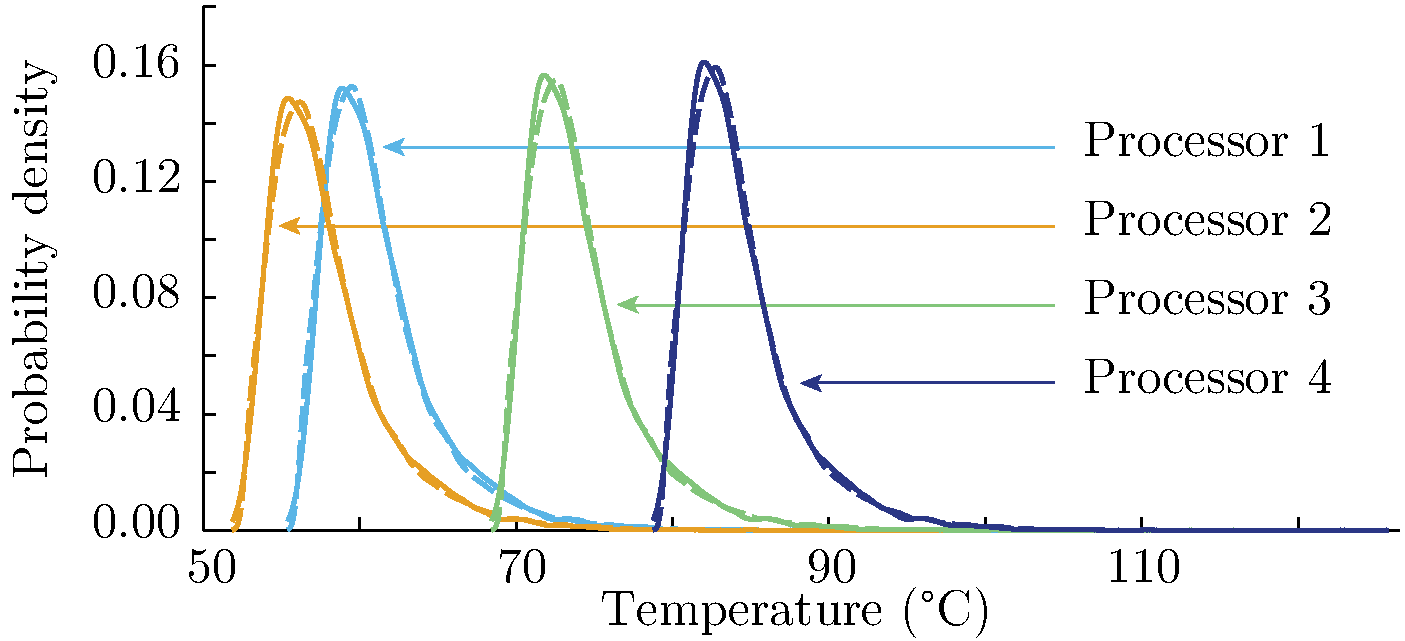
\includegraphics[width=1\ColumnWidth]{include/assets/experimental-results-pdf.pdf}
  \vspace{-2.0em}
  \caption{Probability density functions computed at time 50$\,\text{ms}$ using the proposed framework (the dashed lines) and MC sampling (the solid lines).}
  \flabel{experimental-results-pdf}
\end{figure}

First, we concentrate on the proposed technique and, thus, pay particular attention the columns of \tref{accuracy-eta-0-5} corresponding to high values of $\nsamples$.
It can be seen that the error of the expected value, $\eExp$, is small even for $\pcorder = 1$; more precisely, it is bounded by 0.6\% (see $\eExp$ for $\pcorder \geq 1$ and $\nsamples \geq 10^4$).
The error of the second central moment, $\eVar$, starts from about 67\% for the first-order PC expansions and drops significantly to less than 6\% for the fourth order (see $\eVar$ for $\pcorder \geq 4$ and $\nsamples = 10^5$).
The results of the third error metric, $\ePDF$, allow us to conclude that the \pdfs\ computed by the third-order (and higher) PC expansions closely follow those estimated by the MC technique with large numbers of samples, namely, the observed difference in \tref{accuracy-eta-0-5} is bounded by 2\% (see $\ePDF$ for $\pcorder \geq 3$ and $\nsamples \geq 10^4$).
In order to give a better appreciation of the proximity of the two methods, \fref{experimental-results-pdf} displays an example of the \pdfs\ obtained using our framework with $\pcorder = 4$ (the dashed lines) along with those estimated by the MC approach with $\nsamples = 10^4$ (the solid lines).
Note that this example captures one particular moment of time, and such curves are readily available for all the other steps of the considered time span (here we show the middle).
It can be seen in \fref{experimental-results-pdf} that the empirical \pdfs\ tightly match each other.

Now we take a closer look at the convergence of the MC-based technique.
With this in mind, we focus on the rows of \tref{accuracy-eta-0-5} that correspond to PC expansions of high orders.
Similar to the previous findings, even for low requirements, the error of the expected values estimated by MC sampling is relatively small: it is around 1\% (see $\eExp$ for $\pcorder \geq 4$ and $\nsamples = 10^2$).
At the same time, the case with $\nsamples = 10^2$ has a high error rate in terms of $\eVar$ and $\ePDF$, namely, it is above 38\% for variance and almost 3.5\% for \pdfs\ (see $\eVar$ and $\ePDF$ for $\pcorder \geq 3$ and $\nsamples = 10^2$).
The results of the MC approach with $\nsamples = 10^3$ are reasonably more accurate; however, this trend is compromised by the results in \tref{accuracy-eta-1}.
Specifically, $10^3$ MC samples leave an error of more than 7\% for variance in \tref{accuracy-eta-1} (see $\eVar$ for $\pcorder \geq 4$ and $\nsamples = 10^3$).
Lastly, we note that, for a fixed $\pcorder \geq 4$, $\eVar$ exhibits a considerable decrease in \tref{accuracy-eta-0-5} even when $\nsamples$ transitions from $10^4$ to $10^5$.
The rate of this decrease suggests that $\nsamples = 10^4$ is not sufficient to reach the same accuracy as the one delivered by our framework, and $\nsamples = 10^5$ might not be either.

Finally, we would like mention that the aforementioned conclusions, based on \tref{accuracy-eta-0-5} ($\eta = 0.5$), are directly applicable to \tref{accuracy-eta-0} ($\eta = 0$) and \tref{accuracy-eta-1} ($\eta = 1$).
The only difference is that the average error rates are lower when either of the two correlation kernels dominates.
In particular, according to $\eVar$, the case with $\eta = 1$, which corresponds to the squared exponential kernel, stands out to be the least error prone.
